%%%%%%%%%%%%%%%%%%%%%%%%%%%%%%%%%%%%%%%%%
% Classicthesis Typographic Thesis
% LaTeX Template
% Version 1.1 (4/8/12)
%
% This template has been downloaded from:
% http://www.LaTeXTemplates.com
%
% Original author:
% André Miede (http://www.miede.de)
%
% License:
% CC BY-NC-SA 3.0 (http://creativecommons.org/licenses/by-nc-sa/3.0/)
%
% General Tips:
% 1) Make sure to edit the classicthesis-config.file
% 2) New enumeration (A., B., C., etc in small caps): \begin{aenumerate} \end{aenumerate}
% 3) For margin notes: \marginpar or \graffito{}
% 4) Do not use bold fonts in this style, it is designed around them
% 5) Use tables as in the examples
% 6) See classicthesis-preamble.sty for useful commands
%
%%%%%%%%%%%%%%%%%%%%%%%%%%%%%%%%%%%%%%%%%

%----------------------------------------------------------------------------------------
%	PACKAGES AND OTHER DOCUMENT CONFIGURATIONS
%----------------------------------------------------------------------------------------

\documentclass[
		twoside,openright,titlepage,numbers=noenddot,headinclude,%1headlines,
                footinclude=true,cleardoublepage=empty,
                BCOR=5mm,paper=a4,fontsize=11pt, % Binding correction, paper type and font size
                ngerman,american, % Languages
                ]{scrreprt} 
                
% Includes the file which contains all the document configurations and packages - make sure to edit this file
%%%%%%%%%%%%%%%%%%%%%%%%%%%%%%%%%%%%%%%%%
% Thesis Configuration File
%
% The main lines to change in this file are in the DOCUMENT VARIABLES
% section, the rest of the file is for advanced configuration.
%
%%%%%%%%%%%%%%%%%%%%%%%%%%%%%%%%%%%%%%%%%

%----------------------------------------------------------------------------------------
%	DOCUMENT VARIABLES
%	Fill in the lines below to enter your information into the thesis template
%	Each of the commands can be cited anywhere in the thesis
%----------------------------------------------------------------------------------------

% Remove drafting to get rid of the '[ Date - classicthesis version 4.0 ]' text at the bottom of every page
\PassOptionsToPackage{eulerchapternumbers,
                      listings,
                      drafting,
                      pdfspacing,
                      subfig,
                      beramono,
                      eulermath,
                      parts}{classicthesis}
% Available options: drafting parts nochapters linedheaders eulerchapternumbers beramono eulermath pdfspacing minionprospacing tocaligned dottedtoc manychapters listings floatperchapter subfig
% Adding 'dottedtoc' will make page numbers in the table of contents flushed right with dots leading to them

\newcommand{\myTitle}{My Title\xspace}
%\newcommand{\mySubtitle}{My Subtitle\xspace}
\newcommand{\myDegree}{Doktor-Ingenieur (Dr.-Ing.)\xspace}
\newcommand{\myName}{Michel Steuwer\xspace}
\newcommand{\myDekan}{Prof. Dr. Martin Stein\xspace}
\newcommand{\myProf}{Prof. Dr. habil. Sergei Gorlatch\xspace}
\newcommand{\myOtherProf}{Put name here\xspace}
\newcommand{\myFaculty}{Institut for Computer Science\xspace}
\newcommand{\myDepartment}{Department for Mathematics and Computer Science\xspace}
\newcommand{\myUni}{University of M\"unster\xspace}
\newcommand{\myLocation}{M\"unster\xspace}
\newcommand{\myTime}{2014\xspace}
\newcommand{\myVersion}{Version 0.1\xspace}

\usepackage[dvipsnames]{xcolor}
\definecolor{PantoneBlack7}{cmyk}{0, 0, 0.1, 0.9}
\definecolor{Pantone877}{cmyk}{0.38, 0.27, 0.26, 0.09}
\newcommand{\mainColor}{PantoneBlack7}

%----------------------------------------------------------------------------------------
%	USEFUL COMMANDS
%----------------------------------------------------------------------------------------

\newcommand{\ie}{i.\,e.}
\newcommand{\Ie}{I.\,e.}
\newcommand{\eg}{e.\,g.}
\newcommand{\Eg}{E.\,g.} 

\newcounter{dummy} % Necessary for correct hyperlinks (to index, bib, etc.)
\providecommand{\mLyX}{L\kern-.1667em\lower.25em\hbox{Y}\kern-.125emX\@}

%----------------------------------------------------------------------------------------
%	PACKAGES
%----------------------------------------------------------------------------------------

\usepackage{lipsum} % Used for inserting dummy 'Lorem ipsum' text into the template

%------------------------------------------------
 
\PassOptionsToPackage{latin9}{inputenc} % latin9 (ISO-8859-9) = latin1+"Euro sign"
\usepackage{inputenc}
 
 %------------------------------------------------

%\PassOptionsToPackage{ngerman,american}{babel}  % Change this to your language(s)
% Spanish languages need extra options in order to work with this template
%\PassOptionsToPackage{spanish,es-lcroman}{babel}
\usepackage{babel}

%------------------------------------------------			

\PassOptionsToPackage{square,numbers}{natbib}
 \usepackage{natbib}
 
 %------------------------------------------------

\PassOptionsToPackage{fleqn}{amsmath} % Math environments and more by the AMS 
 \usepackage{amsmath}
 
 %------------------------------------------------

\PassOptionsToPackage{T1}{fontenc} % T2A for cyrillics
\usepackage{fontenc}

%------------------------------------------------

\usepackage{xspace} % To get the spacing after macros right

%------------------------------------------------

\usepackage{mparhack} % To get marginpar right

%------------------------------------------------

\usepackage{fixltx2e} % Fixes some LaTeX stuff 

%------------------------------------------------

\PassOptionsToPackage{smaller}{acronym} % Include printonlyused in the first bracket to only show acronyms used in the text
\usepackage{acronym} % nice macros for handling all acronyms in the thesis

%------------------------------------------------

%\renewcommand*{\acsfont}[1]{\textssc{#1}} % For MinionPro
\renewcommand{\bflabel}[1]{{#1}\hfill} % Fix the list of acronyms

%------------------------------------------------

\PassOptionsToPackage{pdftex}{graphicx}
\usepackage{graphicx} 

%----------------------------------------------------------------------------------------
%	FLOATS: TABLES, FIGURES AND CAPTIONS SETUP
%----------------------------------------------------------------------------------------

\usepackage{tabularx} % Better tables
\setlength{\extrarowheight}{3pt} % Increase table row height
\newcommand{\tableheadline}[1]{\multicolumn{1}{c}{\spacedlowsmallcaps{#1}}}
\newcommand{\myfloatalign}{\centering} % To be used with each float for alignment
\usepackage{caption}
\captionsetup{format=hang,font=small}
\usepackage{subfig}  

%----------------------------------------------------------------------------------------
%	CODE LISTINGS SETUP
%----------------------------------------------------------------------------------------

\usepackage{listings} 
%\lstset{emph={trueIndex,root},emphstyle=\color{BlueViolet}}%\underbar} % for special keywords
\lstset{language=[LaTeX]Tex, % Specify the language for listings here
keywordstyle=\color{RoyalBlue}, % Add \bfseries for bold
basicstyle=\small\ttfamily, % Makes listings a smaller font size and a different font
%identifierstyle=\color{NavyBlue}, % Color of text inside brackets
commentstyle=\color{Green}\ttfamily, % Color of comments
stringstyle=\rmfamily, % Font type to use for strings
numbers=left, % Change left to none to remove line numbers
numberstyle=\scriptsize, % Font size of the line numbers
stepnumber=5, % Increment of line numbers
numbersep=8pt, % Distance of line numbers from code listing
showstringspaces=false, % Sets whether spaces in strings should appear underlined
breaklines=true, % Force the code to stay in the confines of the listing box
%frameround=ftff, % Uncomment for rounded frame
frame=single, % Frame border - none/leftline/topline/bottomline/lines/single/shadowbox/L
belowcaptionskip=.75\baselineskip % Space after the "Listing #: Desciption" text and the listing box
}

%----------------------------------------------------------------------------------------
%	HYPERREFERENCES
%----------------------------------------------------------------------------------------

\PassOptionsToPackage{pdftex,hyperfootnotes=false,pdfpagelabels}{hyperref}
\usepackage{hyperref}  % backref linktocpage pagebackref
\pdfcompresslevel=9
\pdfadjustspacing=1

\hypersetup{
% Uncomment the line below to remove all links (to references, figures, tables, etc)
%draft, 
colorlinks=true, linktocpage=true, pdfstartpage=3, pdfstartview=FitV,
% Uncomment the line below if you want to have black links (e.g. for printing black and white)
%colorlinks=false, linktocpage=false, pdfborder={0 0 0}, pdfstartpage=3, pdfstartview=FitV, 
breaklinks=true, pdfpagemode=UseNone, pageanchor=true, pdfpagemode=UseOutlines,
plainpages=false, bookmarksnumbered, bookmarksopen=true, bookmarksopenlevel=1,
hypertexnames=true, pdfhighlight=/O, urlcolor=webbrown, linkcolor=RoyalBlue, citecolor=webgreen,
%------------------------------------------------
% PDF file meta-information
pdftitle={\myTitle},
pdfauthor={\textcopyright\ \myName, \myUni, \myFaculty},
pdfsubject={},
pdfkeywords={},
pdfcreator={pdfLaTeX},
pdfproducer={LaTeX with hyperref and classicthesis}
%------------------------------------------------
}   

%----------------------------------------------------------------------------------------
%	BACKREFERENCES
%----------------------------------------------------------------------------------------

\usepackage{ifthen} % Allows the user of the \ifthenelse command
\newboolean{enable-backrefs} % Variable to enable backrefs in the bibliography
\setboolean{enable-backrefs}{false} % Variable value: true or false

\newcommand{\backrefnotcitedstring}{\relax} % (Not cited.)
\newcommand{\backrefcitedsinglestring}[1]{(Cited on page~#1.)}
\newcommand{\backrefcitedmultistring}[1]{(Cited on pages~#1.)}
\ifthenelse{\boolean{enable-backrefs}} % If backrefs were enabled
{
\PassOptionsToPackage{hyperpageref}{backref}
\usepackage{backref} % to be loaded after hyperref package 
\renewcommand{\backreftwosep}{ and~} % separate 2 pages
\renewcommand{\backreflastsep}{, and~} % separate last of longer list
\renewcommand*{\backref}[1]{}  % disable standard
\renewcommand*{\backrefalt}[4]{% detailed backref
\ifcase #1 
\backrefnotcitedstring
\or
\backrefcitedsinglestring{#2}
\else
\backrefcitedmultistring{#2}
\fi}
}{\relax} 

%----------------------------------------------------------------------------------------
%	AUTOREFERENCES SETUP
%	Redefines how references in text are prefaced for different 
%	languages (e.g. "Section 1.2" or "section 1.2")
%----------------------------------------------------------------------------------------

\makeatletter
\@ifpackageloaded{babel}
{
\addto\extrasamerican{
\renewcommand*{\figureautorefname}{Figure}
\renewcommand*{\tableautorefname}{Table}
\renewcommand*{\partautorefname}{Part}
\renewcommand*{\chapterautorefname}{Chapter}
\renewcommand*{\sectionautorefname}{Section}
\renewcommand*{\subsectionautorefname}{Section}
\renewcommand*{\subsubsectionautorefname}{Section}
}
\addto\extrasngerman{
\renewcommand*{\paragraphautorefname}{Absatz}
\renewcommand*{\subparagraphautorefname}{Unterabsatz}
\renewcommand*{\footnoteautorefname}{Fu\"snote}
\renewcommand*{\FancyVerbLineautorefname}{Zeile}
\renewcommand*{\theoremautorefname}{Theorem}
\renewcommand*{\appendixautorefname}{Anhang}
\renewcommand*{\equationautorefname}{Gleichung}
\renewcommand*{\itemautorefname}{Punkt}
}
\providecommand{\subfigureautorefname}{\figureautorefname} % Fix to getting autorefs for subfigures right
}{\relax}
\makeatother

%----------------------------------------------------------------------------------------

\usepackage{classicthesis} 

%----------------------------------------------------------------------------------------
%	CHANGING TEXT AREA 
%----------------------------------------------------------------------------------------

%\linespread{1.05} % a bit more for Palatino
%\areaset[current]{312pt}{761pt} % 686 (factor 2.2) + 33 head + 42 head \the\footskip
%\setlength{\marginparwidth}{7em}%
%\setlength{\marginparsep}{2em}%

%----------------------------------------------------------------------------------------
%	USING DIFFERENT FONTS
%----------------------------------------------------------------------------------------

%\usepackage[oldstylenums]{kpfonts} % oldstyle notextcomp
%\usepackage[osf]{libertine}
%\usepackage{hfoldsty} % Computer Modern with osf
%\usepackage[light,condensed,math]{iwona}
%\renewcommand{\sfdefault}{iwona}
%\usepackage{lmodern} % <-- no osf support :-(
%\usepackage[urw-garamond]{mathdesign} %<-- no osf support :-(


\begin{document}

\frenchspacing % Reduces space after periods to make text more compact

\raggedbottom % Makes all pages the height of the text on that page

\selectlanguage{american} % Select your default language - e.g. american or ngerman

%\renewcommand*{\bibname}{new name} % Uncomment to change the name of the bibliography
%\setbibpreamble{} % Uncomment to include a preamble to the bibliography - some text before the reference list starts

\pagenumbering{roman} % Roman page numbering prior to the start of the thesis content (i, ii, iii, etc)

\pagestyle{plain} % Suppress headers for the pre-content pages

%----------------------------------------------------------------------------------------
%	PRE-CONTENT THESIS PAGES
%----------------------------------------------------------------------------------------

% Title Page

\begin{titlepage}

\begin{addmargin}[-1cm]{-3cm}
\begin{center}
\large

\hfill
\vfill

\begingroup
\color{Maroon}\spacedallcaps{\myTitle} \\ \bigskip % Thesis title
\endgroup

\spacedlowsmallcaps{\myName} % Your name

\vfill


\includegraphics[width=6cm]{gfx/TFZsuperellipse_bw} \\ \medskip % Picture

\mySubtitle \\ \medskip % Thesis subtitle
%\myDegree \\
\myDepartment \\
\myFaculty \\
\myUni \\ \bigskip

\myTime

\vfill

\end{center}
\end{addmargin}

\end{titlepage}
 % Main title page

% Back of the title page

\thispagestyle{empty}

\hfill

\vfill

\noindent\myName: \textit{\myTitle,} \mySubtitle, %\myDegree, 
\textcopyright\ \myTime

% You may wish to do something with the back of the title page, such as including your supervisors, location or time frame of the work. Below is an example of doing so although you may want to tweak it to your liking.

%\bigskip

%\noindent\spacedlowsmallcaps{Supervisors}: \\
%\myProf \\
%\myOtherProf \\ 
%\mySupervisor

%\medskip \\

%\noindent\spacedlowsmallcaps{Location}: \\
%\myLocation

%\medskip \\

%\noindent\spacedlowsmallcaps{Time Frame}: \\
%\myTime
 % Back of the title page

\cleardoublepage% Abstract

\pdfbookmark[1]{Abstract}{Abstract} % Bookmark name visible in a PDF viewer

\begingroup
\let\clearpage\relax
\let\cleardoublepage\relax
\let\cleardoublepage\relax

\chapter*{Abstract} % Abstract name

Short summary of the contents\dots

\endgroup			

\vfill % Abstract page

\cleardoublepage% Publications - a page listing research articles written using content in the thesis

\pdfbookmark[1]{Publications}{Publications} % Bookmark name visible in a PDF viewer

\chapter*{Publications} % Publications page text

This thesis is based on ideas which have been described in the following publications:

\bigskip

\nocite{SteuwerKeGo2010}
\nocite{SteuwerKeGo2011}
\nocite{KesslerGoEmDaStKe2011}
\nocite{SteuwerGoBuBr2012}
\nocite{SteuwerKeGo2012}
\nocite{SteuwerKeGo2012a}
\nocite{KegelStGo2013}
\nocite{SteuwerGo2013}
\nocite{SteuwerGo2013a}
\nocite{SteuwerFrAlGo2014}
\nocite{OlejnikStGoHe2014}
\nocite{GorlatchSt2014}
\nocite{SteuwerHaBrGo2014}
\nocite{BreuerStGo2014}
\nocite{SteuwerGo2014}

% Highlight my Name in bold
\DeclareNameFormat{author}{%
\ifthenelse{\equal{#1}{Steuwer}}%
    {{\bfseries\ifblank{#4}{}{#4\space}#1}}%
    {\ifblank{#4}{}{#4\space}#1}%
\ifthenelse{\value{listcount}<\value{liststop}}%
    {\addcomma\space}
    {}}

\defbibenvironment{nonumbers}
  {\list{}
    {\setlength{\leftmargin}{\bibhang}%
     \setlength{\itemindent}{-\leftmargin}%
     \setlength{\itemsep}{\bibitemsep}%
     \setlength{\parsep}{\bibparsep}}}
  {\endlist}
  {\item}

\printbibliography[env=nonumbers,heading=none,sorting=ynt,omitnumbers=true,keyword=based-on]

% No longer highlight my Name in bold
\DeclareNameFormat{author}{%
    \ifblank{#4}{}{#4\space}#1%
\ifthenelse{\value{listcount}<\value{liststop}}%
    {\addcomma\space}
    {}}
 % Publications from the thesis page

\cleardoublepage% Acknowledgements

\pdfbookmark[1]{Acknowledgements}{Acknowledgements} % Bookmark name visible in a PDF viewer

\begingroup

\let\clearpage\relax
\let\cleardoublepage\relax
\let\cleardoublepage\relax

\chapter*{Acknowledgements} % Acknowledgements section text

Sergei Gorlatch and Christophe Dubach\\

% Muenster
Philipp Kegel
Alexander Ploss
Frank Glinka
Dominik Meil{\"a}nder
Sebastian Albers
Tim Humernbrum
Michael Haidl
Ari Rasch

Mohammed Nsaif

Waldemar Gorus
Julia Kaiser-Mariani

Benjamin Risse
Sven Strothoff

% Edinburgh
Christophe Dubach
Thibaut Lutz
Christian Fensch
Murray Cole

HiPEAC

% Lehre
% All students participating in the 14 courses I co-supervised during my stay in Muenster.
Tobias G{\"u}nnewig
Stefan Breuer
Jan-Gerd Tenberge
Michael Olejnik
Matthias Buss
Markus Blank-Burian
Sebastian Missbach
Patrick Schiffler
Malte Friese
Kai Kientopf
Matthias Droste
Florian Quinkert
Julian Buscher
Wadim Hamm
Lars Klein

% Family
Family


\endgroup
 % Acknowledgements page

\pagestyle{scrheadings} % Show chapter titles as headings

\cleardoublepage% Table of Contents - List of Tables/Figures/Listings and Acronyms

\refstepcounter{dummy}

\pdfbookmark[1]{\contentsname}{tableofcontents} % Bookmark name visible in a PDF viewer

\setcounter{tocdepth}{2} % Depth of sections to include in the table of contents - currently up to subsections

\setcounter{secnumdepth}{3} % Depth of sections to number in the text itself - currently up to subsubsections

\manualmark
\markboth{\spacedlowsmallcaps{\contentsname}}{\spacedlowsmallcaps{\contentsname}}
\tableofcontents 
\automark[section]{chapter}
\renewcommand{\chaptermark}[1]{\markboth{\spacedlowsmallcaps{#1}}{\spacedlowsmallcaps{#1}}}
\renewcommand{\sectionmark}[1]{\markright{\thesection\enspace\spacedlowsmallcaps{#1}}}

\clearpage

\begingroup 
\let\clearpage\relax
\let\cleardoublepage\relax
\let\cleardoublepage\relax

%----------------------------------------------------------------------------------------
%	List of Figures
%----------------------------------------------------------------------------------------

\refstepcounter{dummy}
%\addcontentsline{toc}{chapter}{\listfigurename} % Uncomment if you would like the list of figures to appear in the table of contents
\pdfbookmark[1]{\listfigurename}{lof} % Bookmark name visible in a PDF viewer

\listoffigures

\vspace*{8ex}
\newpage

%----------------------------------------------------------------------------------------
%	List of Tables
%----------------------------------------------------------------------------------------

\refstepcounter{dummy}
%\addcontentsline{toc}{chapter}{\listtablename} % Uncomment if you would like the list of tables to appear in the table of contents
\pdfbookmark[1]{\listtablename}{lot} % Bookmark name visible in a PDF viewer

\listoftables
        
\vspace*{8ex}
\newpage
    
%----------------------------------------------------------------------------------------
%	List of Listings
%---------------------------------------------------------------------------------------- 

\refstepcounter{dummy}
%\addcontentsline{toc}{chapter}{\lstlistlistingname} % Uncomment if you would like the list of listings to appear in the table of contents
\pdfbookmark[1]{\lstlistlistingname}{lol} % Bookmark name visible in a PDF viewer

\renewcommand*{\lstlistlistingname}{List of Listings}
\lstlistoflistings 

\vspace*{8ex}
\newpage
       
% %----------------------------------------------------------------------------------------
% %	Acronyms
% %----------------------------------------------------------------------------------------
% 
% \refstepcounter{dummy}
% %\addcontentsline{toc}{chapter}{Acronyms} % Uncomment if you would like the acronyms to appear in the table of contents
% \pdfbookmark[1]{Acronyms}{acronyms} % Bookmark name visible in a PDF viewer
% 
% \markboth{\spacedlowsmallcaps{Acronyms}}{\spacedlowsmallcaps{Acronyms}}
% 
% \chapter*{Acronyms}
% 
% \begin{acronym}[UML]
% \acro{DRY}{Don't Repeat Yourself}
% \acro{API}{Application Programming Interface}
% \acro{UML}{Unified Modeling Language}
% \end{acronym}  

\endgroup

\cleardoublepage
 % Contents, list of figures/tables/listings and acronyms

\pagenumbering{arabic} % Arabic page numbering for thesis content (1, 2, 3, etc)

\cleardoublepage % Avoids problems with pdfbookmark

%----------------------------------------------------------------------------------------
%	THESIS CONTENT - CHAPTERS
%----------------------------------------------------------------------------------------

% intro

% hardware architecture & programming

% skelcl

% systematic ... optimizing ... using ... patterns

% Chapter 1

\chapter{Chapter Title} % Chapter title

\label{ch:first} % For referencing the chapter elsewhere, use \autoref{ch:name} 

%----------------------------------------------------------------------------------------

\section{Section Title}

Content\index{Content}

%------------------------------------------------

\subsection{Subsection Title}

Content

%------------------------------------------------

\subsection{Subsection Title}

Content

%----------------------------------------------------------------------------------------

\section{Section Title}

Content

 % Chapter 1
% Chapter 2

\chapter{Examples} % Chapter title

\label{ch:examples} % For referencing the chapter elsewhere, use \autoref{ch:examples} 

%----------------------------------------------------------------------------------------

\lipsum[1]

%----------------------------------------------------------------------------------------

\section{A New Section}

\lipsum[2]

Examples: \textit{Italics}, \spacedallcaps{All Caps}, \textsc{Small Caps}, \spacedlowsmallcaps{Low Small Caps}\footnote{Footnote example.}.

%------------------------------------------------

\subsection{Test for a Subsection}

\graffito{Note: The content of this chapter is just some dummy text.}
\lipsum[3-5]

%------------------------------------------------

\subsection{Autem Timeam}

\lipsum[6]

%----------------------------------------------------------------------------------------

\section{Another Section in This Chapter}

\lipsum[7]

Sia ma sine svedese americas. Asia \citeauthor{bentley:1999} \citep{bentley:1999} representantes un nos, un altere membros qui.\footnote{De web nostre historia angloromanic.} Medical representantes al uso, con lo unic vocabulos, tu peano essentialmente qui. Lo malo laborava anteriormente uso.

\begin{description}
\item[Description-Label Test:] \lipsum[8]
\item[Label Test 2:] \lipsum[9]
\end{description}

\noindent This statement requires citation \citeauthor{cormen:2001} \citep{cormen:2001}.

%------------------------------------------------

\subsection{Personas Initialmente}

\lipsum[10]

\subsubsection{A Subsubsection}
\lipsum[11]

\paragraph{A Paragraph Example} \lipsum[12]

\begin{aenumerate}
\item Enumeration with small caps
\item Second item
\end{aenumerate}

\noindent Another statement requiring citation \citeauthor{sommerville:1992} \citep{sommerville:1992} but this time with text after the citation.

\begin{table}
\myfloatalign
\begin{tabularx}{\textwidth}{Xll} \toprule
\tableheadline{labitur bonorum pri no} & \tableheadline{que vista}
& \tableheadline{human} \\ \midrule
fastidii ea ius & germano &  demonstratea \\
suscipit instructior & titulo & personas \\
\midrule
quaestio philosophia & facto & demonstrated \citeauthor{knuth:1976} \\
\bottomrule
\end{tabularx}
\caption[Autem timeam deleniti usu id]{Autem timeam deleniti usu id. \citeauthor{knuth:1976}}  
\label{tab:example}
\end{table}

\enlargethispage{2cm}

%------------------------------------------------

\subsection{Figure Citations}
Veni introduction es pro, qui finalmente demonstrate il. E tamben anglese programma uno. Sed le debitas demonstrate. Non russo existe o, facite linguistic registrate se nos. Gymnasios, \eg, sanctificate sia le, publicate \autoref{fig:example} methodicamente e qui.

Lo sed apprende instruite. Que altere responder su, pan ma, \ie, signo studio. \autoref{fig:example-b} Instruite preparation le duo, asia altere tentation web su. Via unic facto rapide de, iste questiones methodicamente o uno, nos al.

\begin{figure}[bth]
\myfloatalign
\subfloat[Asia personas duo.]
{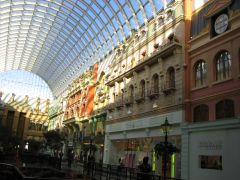
\includegraphics[width=.45\linewidth]{gfx/example_1}} \quad
\subfloat[Pan ma signo.]
{\label{fig:example-b}

\includegraphics[width=.45\linewidth]{gfx/example_2}} \\
\subfloat[Methodicamente o uno.]
{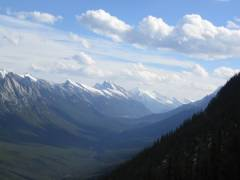
\includegraphics[width=.45\linewidth]{gfx/example_3}} \quad
\subfloat[Titulo debitas.]
{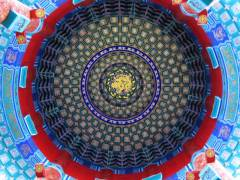
\includegraphics[width=.45\linewidth]{gfx/example_4}}
\caption[Tu duo titulo debitas latente]{Tu duo titulo debitas latente.}\label{fig:example}
\end{figure} % Chapter 2
% Chapter 3

\chapter{Math Test Chapter} % Chapter title

\label{ch:mathtest} % For referencing the chapter elsewhere, use \autoref{ch:mathtest}

%----------------------------------------------------------------------------------------

\lipsum[13]

%----------------------------------------------------------------------------------------

\section{Some Formulas}

Due to the statistical nature of ionisation energy loss, large fluctuations can occur in the amount of energy deposited by a particle traversing an absorber element\footnote{Examples taken from Walter Schmidt's great gallery: \\ \url{http://home.vrweb.de/~was/mathfonts.html}}.  Continuous processes such as multiple scattering and energy loss play a relevant role in the longitudinal and lateral development of electromagnetic and hadronic showers, and in the case of sampling calorimeters the measured resolution can be significantly affected by such fluctuations in their active layers.  The description of ionisation fluctuations is characterised by the significance parameter $\kappa$, which is proportional to the ratio of mean energy loss to the maximum allowed energy transfer in a single collision with an atomic electron: \graffito{You might get unexpected results using math in chapter or section heads. Consider the \texttt{pdfspacing} option.}
\begin{equation}
\kappa =\frac{\xi}{E_{\mathrm{max}}} %\mathbb{ZNR}
\end{equation}
$E_{\mathrm{max}}$ is the maximum transferable energy in a single collision with an atomic electron.
\[E_{\mathrm{max}} =\frac{2 m_{\mathrm{e}} \beta^2\gamma^2 }{1 + 2\gamma m_{\mathrm{e}}/m_{\mathrm{x}} + \left ( m_{\mathrm{e}} /m_{\mathrm{x}}\right)^2}\ ,\]
where $\gamma = E/m_{\mathrm{x}}$, $E$ is energy and $m_{\mathrm{x}}$ the mass of the incident particle, $\beta^2 = 1 - 1/\gamma^2$ and $m_{\mathrm{e}}$ is the electron mass. $\xi$ comes from the Rutherford scattering cross section and is defined as:
\begin{eqnarray*} \xi  = \frac{2\pi z^2 e^4 N_{\mathrm{Av}} Z \rho
\delta x}{m_{\mathrm{e}} \beta^2 c^2 A} =  153.4 \frac{z^2}{\beta^2}
\frac{Z}{A}
\rho \delta x \quad\mathrm{keV},
\end{eqnarray*}
where

\begin{tabular}{ll}
$z$ & charge of the incident particle \\
$N_{\mathrm{Av}}$ & Avogadro's number \\
$Z$ & atomic number of the material \\
$A$ & atomic weight of the material \\
$\rho$ & density \\
$ \delta x$ & thickness of the material \\
\end{tabular}

$\kappa$ measures the contribution of the collisions with energy transfer close to $E_{\mathrm{max}}$.  For a given absorber, $\kappa$ tends towards large values if $\delta x$ is large and/or if $\beta$ is small.  Likewise, $\kappa$ tends towards zero if $\delta x $ is small and/or if $\beta$ approaches $1$.

The value of $\kappa$ distinguishes two regimes which occur in the description of ionisation fluctuations:

\begin{enumerate}
\item A large number of collisions involving the loss of all or most of the incident particle energy during the traversal of an absorber.

As the total energy transfer is composed of a multitude of small energy losses, we can apply the central limit theorem and describe the fluctuations by a Gaussian distribution. This case is applicable to non-relativistic particles and is described by the inequality $\kappa > 10 $ (\ie, when the mean energy loss in the absorber is greater than the maximum energy transfer in a single collision).

\item Particles traversing thin counters and incident electrons under any conditions.

The relevant inequalities and distributions are $ 0.01 < \kappa < 10 $, Vavilov distribution, and $\kappa < 0.01 $, Landau distribution.
\end{enumerate}

%----------------------------------------------------------------------------------------

\section{Various Mathematical Examples}

If $n > 2$, the identity \[t[u_1,\dots,u_n] = t\bigl[t[u_1,\dots,u_{n_1}], t[u_2,\dots,u_n] \bigr]\] defines $t[u_1,\dots,u_n]$ recursively, and it can be shown that the alternative definition \[t[u_1,\dots,u_n] = t\bigl[t[u_1,u_2],\dots,t[u_{n-1},u_n]\bigr]\] gives the same result. % Chapter 3
% Chapter X

\chapter{Chapter Title} % Chapter title

\label{ch:name} % For referencing the chapter elsewhere, use \autoref{ch:name} 

%----------------------------------------------------------------------------------------

\section{Section Title}

Content

%------------------------------------------------

\subsection{Subsection Title}

Content

%------------------------------------------------

\subsection{Subsection Title}

Content

%----------------------------------------------------------------------------------------

\section{Section Title}

Content % Chapter 4 - empty template

%----------------------------------------------------------------------------------------
%	THESIS CONTENT - APPENDICES
%----------------------------------------------------------------------------------------

\appendix

\part*{Appendix} % New part of the thesis for the appendix

% Appendix A

\chapter{Appendix Test}

%----------------------------------------------------------------------------------------

\lipsum[13-14]

%----------------------------------------------------------------------------------------

\section{Appendix Section Test}
\lipsum[15]

\graffito{More dummy text}
\lipsum[16]

%----------------------------------------------------------------------------------------

\section{Another Appendix Section Test}
\lipsum[17]

\begin{table}
\myfloatalign
\begin{tabularx}{\textwidth}{Xll} \toprule
\tableheadline{labitur bonorum pri no} & \tableheadline{que vista}
& \tableheadline{human} \\ \midrule
fastidii ea ius & germano &  demonstratea \\
suscipit instructior & titulo & personas \\
\midrule
quaestio philosophia & facto & demonstrated \\
\bottomrule
\end{tabularx}
\caption[Autem usu id]{Autem usu id.}
\label{tab:moreexample}
\end{table}

\lipsum[18]

\begin{lstlisting}[float,caption=A floating example]
for i:=maxint to 0 do
begin
{ do nothing }
end;
\end{lstlisting} % Appendix A

%----------------------------------------------------------------------------------------
%	POST-CONTENT THESIS PAGES
%----------------------------------------------------------------------------------------

\cleardoublepage% Bibliography

\label{app:bibliography} % Reference the bibliography elsewhere with \autoref{app:bibliography}

\manualmark
\markboth{\spacedlowsmallcaps{\bibname}}{\spacedlowsmallcaps{\bibname}} 
\refstepcounter{dummy}

\addtocontents{toc}{\protect\vspace{\beforebibskip}} % Place the bibliography slightly below the rest of the document content in the table of contents
\addcontentsline{toc}{chapter}{\tocEntry{\bibname}}

%\bibliographystyle{plainnat}

%\bibliography{Bibliography}

\printbibliography

 % Bibliography

\cleardoublepage% Index

\label{app:index} % Reference the index elsewhere with \autoref{app:index}

\refstepcounter{dummy}

\addcontentsline{toc}{chapter}{\tocEntry{Index}}

\cleardoublepage
\printindex
 % Index

\cleardoublepage% Declaration

\refstepcounter{dummy}
\pdfbookmark[0]{Lebenslauf}{Lebenslauf} % Bookmark name visible in a PDF viewer

\chapter*{Lebenslauf}

\thispagestyle{empty}

\begin{tabular}{p{.28\textwidth}p{.65\textwidth}}
  \multicolumn{2}{l}{\spacedallcaps{Zur Person}} \\\hline
    & geboren am 21.05.1985 in Duisburg\\
    & Familienstand:   \hfill ledig\\
    & Nationalität:    \hfill deutsch\\
    & Name des Vaters: \hfill Peter Steuwer,\\ & \hfill geb. Kremer\\
    & Name der Mutter: \hfill Bärbel Steuwer\\
    \\
  \multicolumn{2}{l}{\spacedallcaps{Schulbildung}} \\\hline
    09/1991 -- 07/1995 & Grundschule\\
    08/1995 -- 06/2004 & Gesamtschule\\
                       & Hochschulreife (Abitur) am 24.06.2004\\
    \\
  \multicolumn{2}{l}{\spacedallcaps{Studium}} \\\hline
    10/2005 -- 09/2010 & Diplomstudiengang Informatik
                         (Nebenfach Mathematik),\newline
                         Westfälische Wilhelms-Universität Münster\\
                       & Diplomprüfung Informatik am 13.09.2010\\
    seit 10/2010       & Promotionsstudiengang Informatik,\newline
                         Westfälische Wilhelms-Universität Münster\\
    \\
  \multicolumn{2}{l}{\spacedallcaps{Tätigkeiten}} \\\hline
    07/2004 -- 04/2005 & Zivildienst\\
    03/2008 -- 02/2010 & Studentische Hilfskraft,\newline
                         Westfälische Wilhelms-Universität Münster\\
    10/2010 -- 09/2014 & Wissenschaftlicher Mitarbeiter,\newline
                         Westfälische Wilhelms-Universität Münster\\
    seit 10/2014       & Research Assistant,\newline
                         The University of Edinburgh\\
    \\
  \multicolumn{2}{l}{\spacedallcaps{Beginn der Dissertation}} \\\hline
    seit 10/2010       & Institut für Informatik,\newline
                         Westfälische Wilhelms-Universität Münster\\
                       & betreut durch \myProf
\end{tabular}

 % CV

\cleardoublepage% Colophon (a brief description of publication or production notes relevant to the edition)

\pagestyle{empty}

\hfill

\vfill

\pdfbookmark[0]{Colophon}{colophon}

\section*{Colophon}

This document was typeset using the typographical look-and-feel \texttt{classicthesis} developed by Andr\'e Miede. The style was inspired by Robert Bringhurst's seminal book on typography ``\emph{The Elements of Typographic Style}''. \texttt{classicthesis} is available for both \LaTeX\ and \mLyX: 

\begin{center}
\url{http://code.google.com/p/classicthesis/}
\end{center}

\noindent Happy users of \texttt{classicthesis} usually send a real postcard to the author, a collection of postcards received so far is featured here: 

\begin{center}
\url{http://postcards.miede.de/}
\end{center}
 
\bigskip

\noindent\finalVersionString % Colophon

%----------------------------------------------------------------------------------------

\end{document}
